% pdflatex presentation

\documentclass[svgnames]{beamer}
\usepackage[utf8]{inputenc}
\usepackage[T1]{fontenc}
\usepackage[sfdefault,scaled=.85,lining]{FiraSans}
\usepackage[scaled=0.85,lining]{FiraMono}
\usepackage{newtxsf}
\usepackage{rotating}
\usepackage{listings}
\usepackage{hyperref}

\usetheme{default}
\setbeamertemplate{navigation symbols}
{%
%  \hspace{3em}
%  \vbox{%
%  \hbox{\insertslidenavigationsymbol}
%  \hbox{\insertframenavigationsymbol}
%  \hbox{\insertbackfindforwardnavigationsymbol}
%  \vspace{2em}}
}

\setbeamerfont{frametitle}{family=\sffamily\firamedium}
\setbeamercolor{alerted text}{fg=red!70!black}
\setbeamercolor{structure}{fg=Navy}
\setbeamertemplate{section in toc shaded}[default][30]


\hypersetup{%
  pdftitle={Teaching programming with Jupyterhub and Nbgrader}
  ,pdfauthor={Gert-Ludwig Ingold <gert.ingold@physik.uni-augsburg.de>}
  ,pdfsubject={Talk at EuroSciPy 2018, Trento 31.8.2018}
  ,pdfkeywords={Python, Jupyterhub, nbgrader, education, EuroSciPy}
}

\definecolor{positive}{rgb}{0, 0.5, 0}
\definecolor{negative}{rgb}{0.7, 0, 0}
\definecolor{myred}{rgb}{0.8, 0, 0}
\definecolor{mygreen}{rgb}{0, 0.6, 0}
\definecolor{myblue}{rgb}{0, 0, 0.8}

\newcommand\but{\alert{\textit{but}} }

\graphicspath{{./images/}}

\begin{document}

\begin{frame}[t]
 \vspace{1.5truecm}
 \begin{center}
  \structure{\huge\textbf{Teaching programming with}}\\[0.2truecm]
  \structure{\huge\textbf{Jupyterhub and Nbgrader}}\\[0.8truecm]
  \structure{\Large Gert-Ludwig Ingold}\\[0.1truecm]
  \structure{\large Universität Augsburg}
 \end{center}
\end{frame}

\begin{frame}{About me}
 \begin{itemize}
  \item theoretical physicist at the Universität Augsburg
  \item teaching programming to physicists and materials scientists\\
	since 2010, typically 10+ students
  \item in two years: mandatory course for 100+ students $\rightarrow$
	  \structure{nbgrader}
  \item involved in two Erasmus+ projects on education and computing
	\begin{itemize}
         \item iCSE4school (2015--2017)
	 \item Juypter@edu (2017--2019)
	\end{itemize}
 \end{itemize}

 \vspace{0.8truecm}
 \structure{Jupyter@edu}\hspace{4.7truecm}%
 \raisebox{-0.7truecm}{
\includegraphics[width=0.37\textwidth]{EU_flag-Erasmus__vect_POS}}

 \vspace{-0.7truecm}
 \begin{itemize}
  \item University of Silesia, Poland (Leader)
  \item Universität Augsburg, Germany
  \item Universidade Portucalense Infante D. Henrique, Portugal
  \item European University Cyprus, Cyprus
 \end{itemize}
\end{frame}

\begin{frame}{nbgrader}
 \begin{center}
 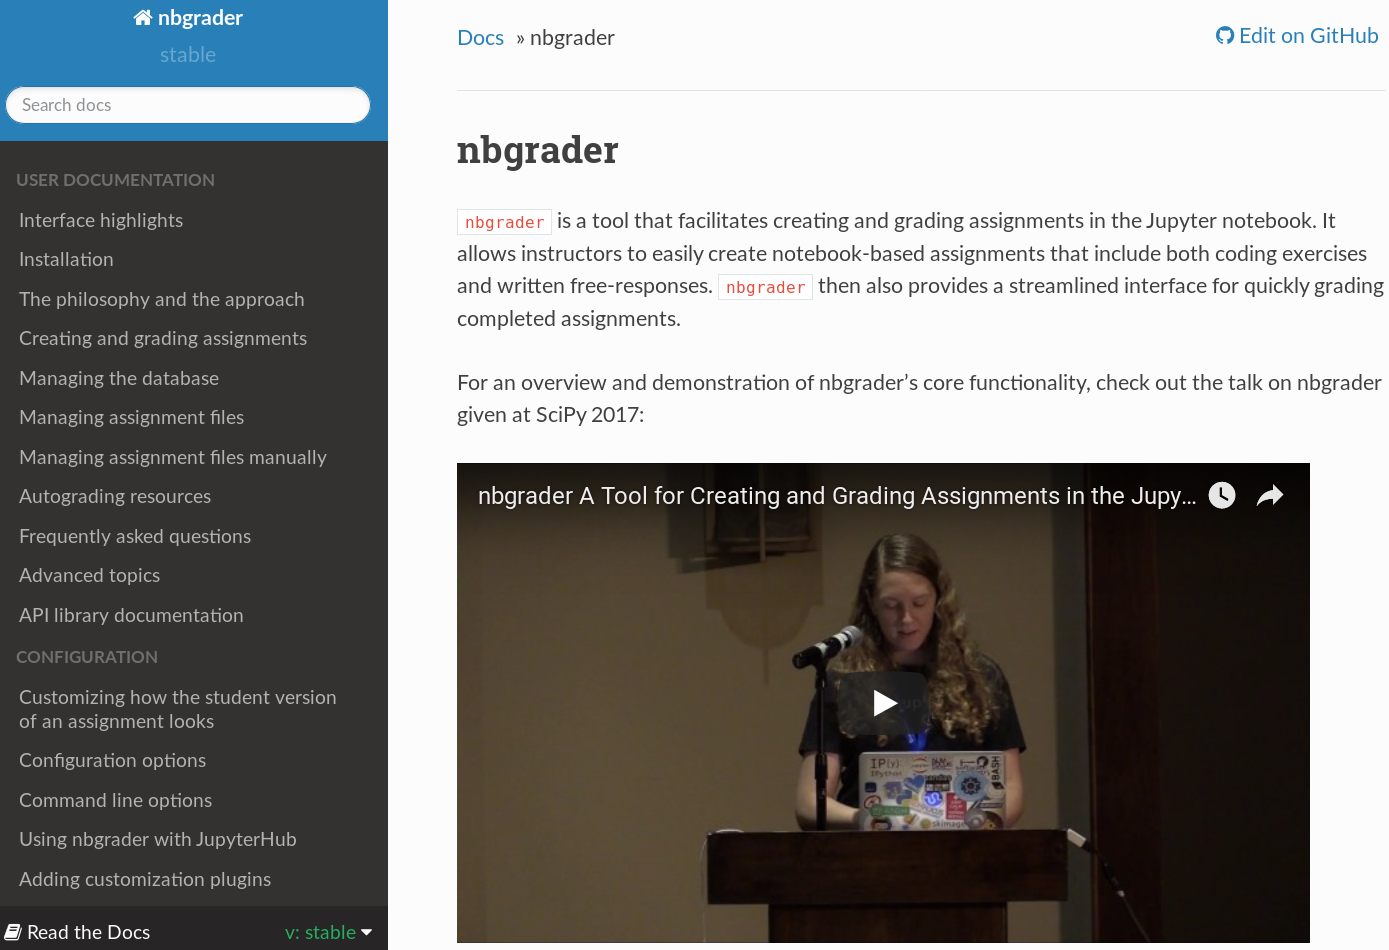
\includegraphics[width=\textwidth]{nbgrader}
 \end{center}

 \url{nbgrader.readthedocs.io}\qquad \url{github.com/jupyter/nbgrader/}
\end{frame}

\begin{frame}
 \begin{center}
  \begin{minipage}{0.6\textwidth}
   \tableofcontents
  \end{minipage}
 \end{center}
\end{frame}

\section{Jupyterhub and Jupyter notebooks}

\begin{frame}
 \begin{center}
  \begin{minipage}{0.6\textwidth}
   \tableofcontents[currentsection]
  \end{minipage}
 \end{center}
\end{frame}

\begin{frame}{Jupyterhub and nbgrader}

 \begin{center}
 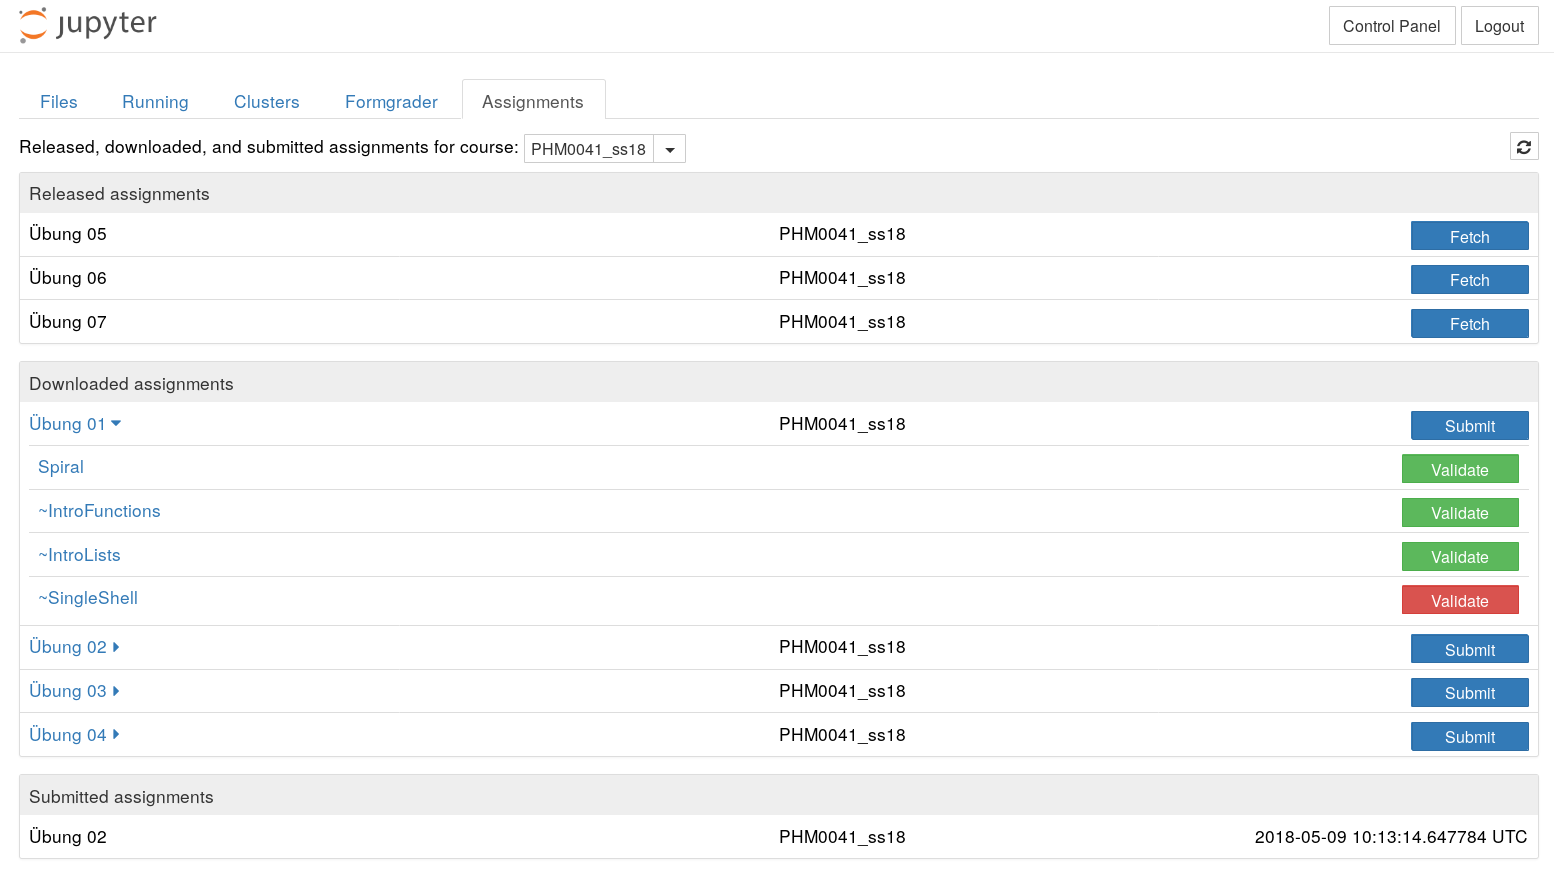
\includegraphics[width=0.9\textwidth]{jupyterhub_nbgrader}
 \end{center}
 \begin{itemize}
  \item easily accessible interface to problem sets
  \item no need to install Python on local computer
  \item consistent working environment for all students
  \item \but may be beginners should gather experience with Python
	on their own computer
 \end{itemize}
\end{frame}

\begin{frame}{Jupyter notebooks or something else?}
 \begin{columns}
  \begin{column}{0.6\textwidth}
   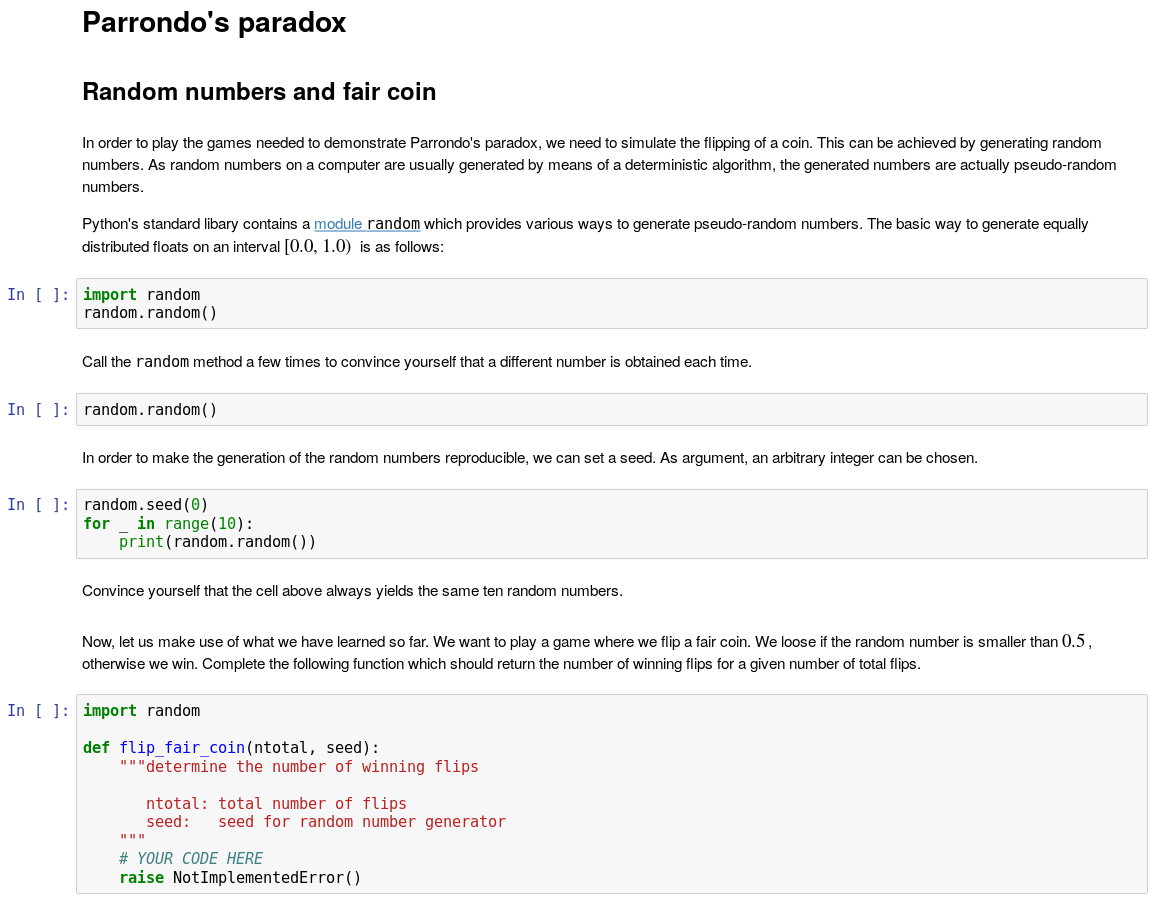
\includegraphics[width=\textwidth]{notebook}
  \end{column}%
  \begin{column}{0.4\textwidth}
   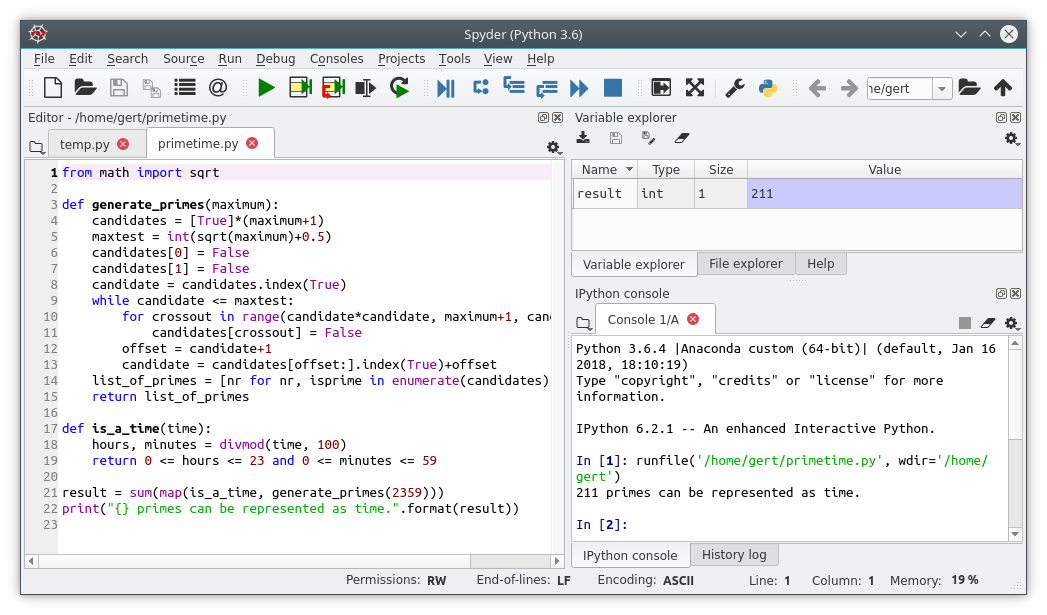
\includegraphics[width=\textwidth]{spyder}

   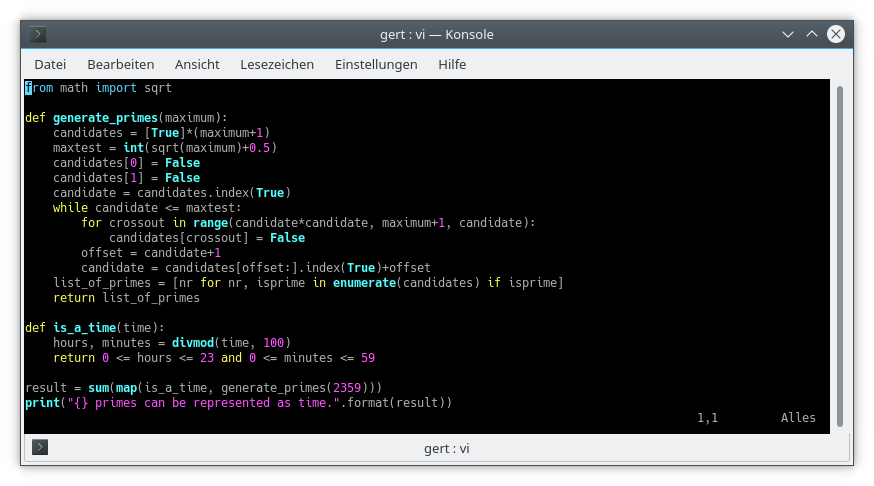
\includegraphics[width=\textwidth]{vim}
  \end{column}
 \end{columns}

 \vspace{0.5truecm}
 \begin{itemize}
  \item notebook allows to guide students through a problem set
  \item students might think that programming in Python implies
	working with a Jupyter notebook
 \end{itemize}
\end{frame}

\section{grading}

\begin{frame}
 \begin{center}
  \begin{minipage}{0.6\textwidth}
   \tableofcontents[currentsection]
  \end{minipage}
 \end{center}
\end{frame}

\begin{frame}{Grading}
 \begin{center}
  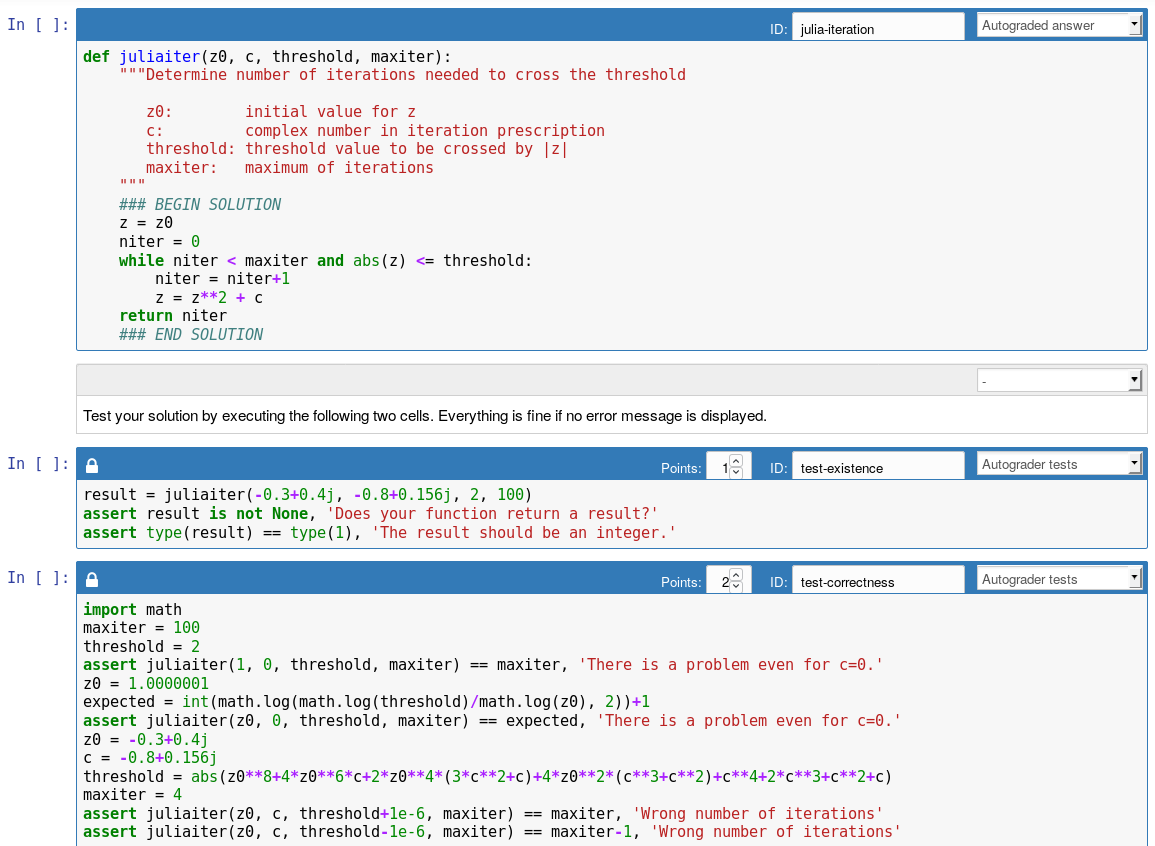
\includegraphics[width=0.8\textwidth]{answer_tests}
 \end{center}
 \begin{itemize}
  \item autograded answer
  \item autograder tests
  \item manually graded answer
 \end{itemize}
\end{frame}

\begin{frame}{Functions}
 \begin{center}
  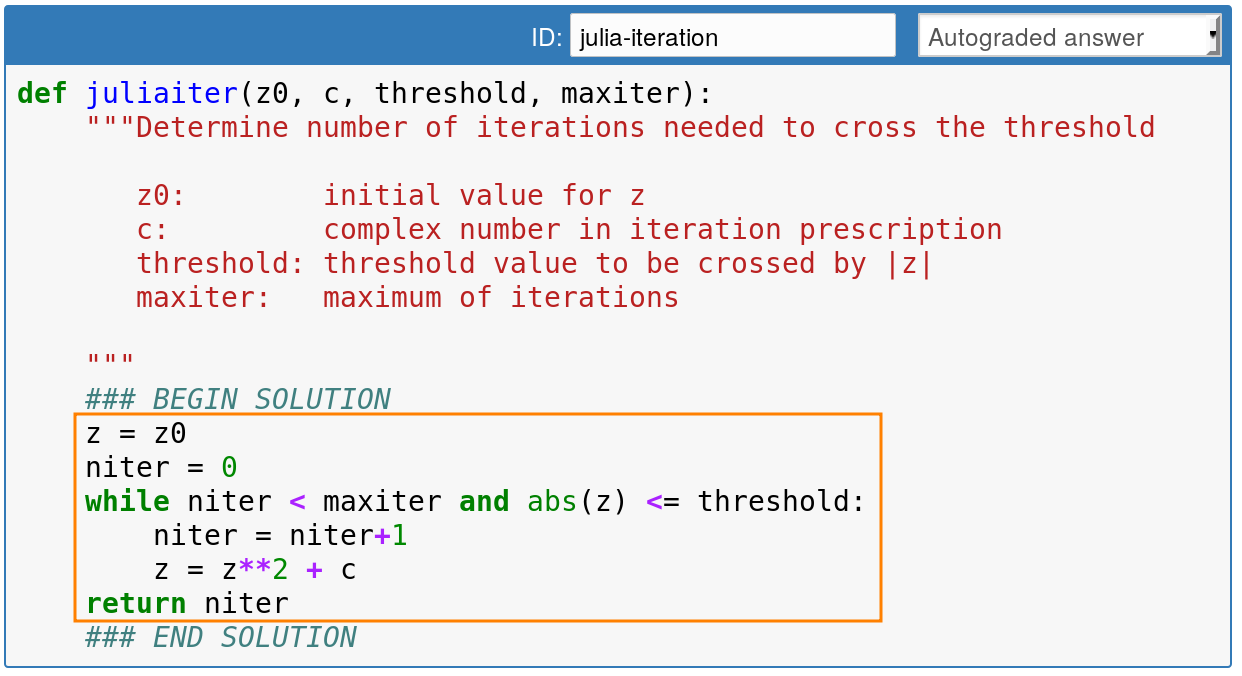
\includegraphics[width=0.7\textwidth]{answer_tests_function}
 \end{center}

 \vspace{-0.4truecm}
 \begin{itemize}
  \item need to introduce functions very early in the course\\
	\but special aspects (no arguments, no return value, default arguments,
	keyword arguments, \dots) not needed
  \item students get used to logically structured code early on\\
	\but they do not do it themselves
  \item include docstrings to make task well defined\\
	students get used to the idea that a function contains a docstring\\
        \but they are not writing the docstring by themselves
 \end{itemize}
\end{frame}

\begin{frame}{Grading with tests}
 \begin{itemize}
  \item test-driven development\\
	\but tests are not developed by the students
  \item tests allow to give feedback through error messages\\
	\but students tend to rely on this feedback instead of developing their
	own critical view on their code
  \item ``Stupid mistakes'' will be made not only at the beginning
	\begin{itemize}
         \item ``trivial'' standard tests (are results returned, do they have the correct type, \dots?)
	 \item + tests of specific functionality which should not disclose the solution
	\end{itemize}
 \end{itemize}
 \begin{center}
  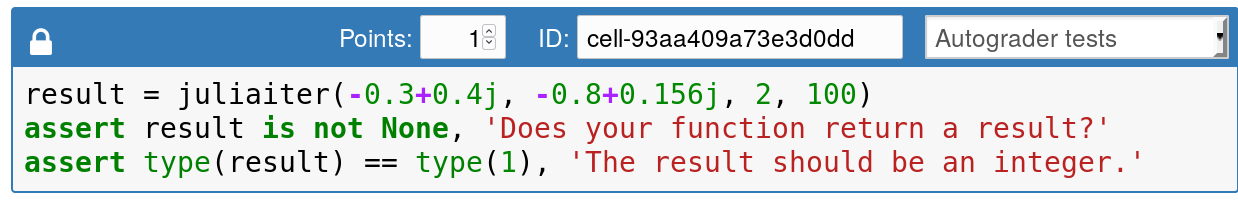
\includegraphics[width=\textwidth]{answer_tests_unittest1}
 \end{center}
\end{frame}

\section{branching paths}

\begin{frame}
 \begin{center}
  \begin{minipage}{0.6\textwidth}
   \tableofcontents[currentsection]
  \end{minipage}
 \end{center}
\end{frame}

\begin{frame}{Coping with heterogeneity}
 \begin{itemize}
  \item students without programming experience and (sometimes) code writing apprehension
  \item students with knowledge in another programming language\\
	code often does not look very pythonic\\
	example: loop over objects vs. loop over indices
 \end{itemize}

 students with programming experience should not be bored and should obtain an interesting result from their code

 \begin{itemize}
  \item \but scientific applications are often considered as an extra mental burden
 \end{itemize}
\end{frame}

\begin{frame}{Examples of problem sets}

 \vspace{-0.7truecm}
 \begin{columns}[t]
  \begin{column}{0.5\textwidth}
   \begin{center}
    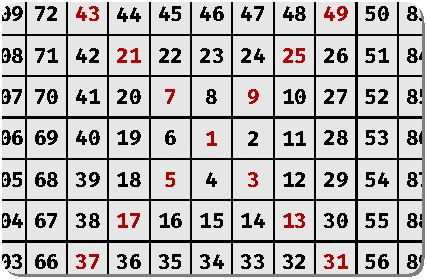
\includegraphics[width=0.8\textwidth]{spiral}

    selected problems from\\[-0.05truecm] Project Euler (\url{projecteuler.net})
   \end{center}
  \end{column}%
  \begin{column}{0.5\textwidth}
   \begin{center}
    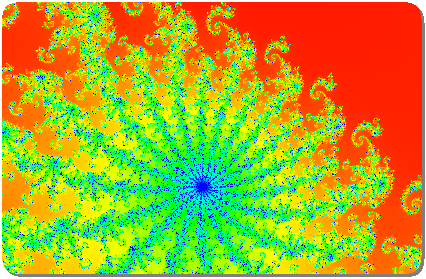
\includegraphics[width=0.8\textwidth]{julia}

    Julia set
   \end{center}
  \end{column}%
 \end{columns}

 \begin{columns}[t]
  \begin{column}{0.5\textwidth}
   \begin{center}
    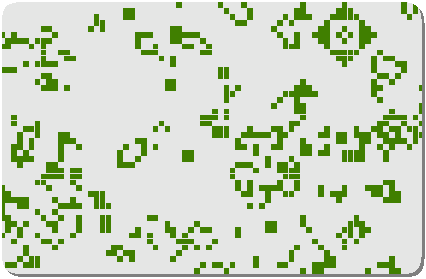
\includegraphics[width=0.8\textwidth]{conway}

    Conway's game of life
   \end{center}
  \end{column}%
  \begin{column}{0.5\textwidth}
   \begin{center}
    
\includegraphics[width=0.8\textwidth]{pi}

    $\pi$ to a few thousand digits
   \end{center}
  \end{column}%
 \end{columns}

 \vspace{0.4truecm}
 {\scriptsize\url{https://github.com/marcinofulus/jupyter4edu/tree/master/augsburg/exercises}}
\end{frame}

\begin{frame}{Branching paths}
 \only<1>{%
  \begin{columns}
   \begin{column}{0.3\textwidth}
    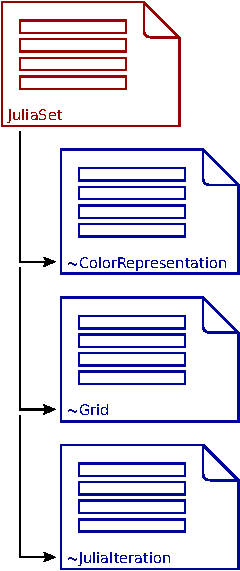
\includegraphics[height=0.8\textheight]{branching_1}
   \end{column}%
   \begin{column}{0.7\textwidth}
    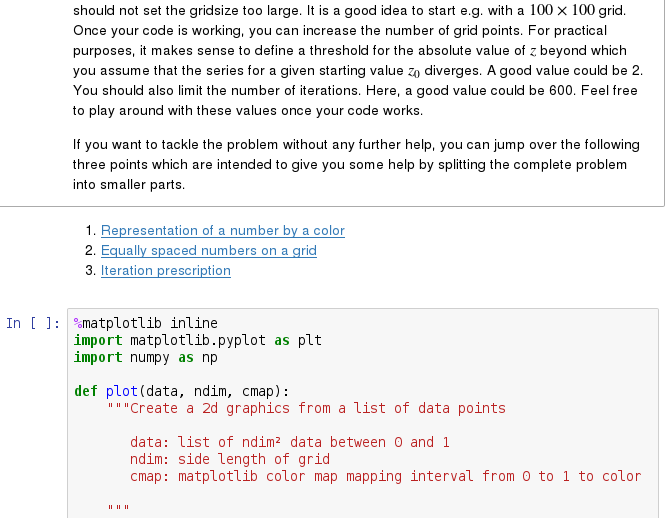
\includegraphics[width=\textwidth]{JuliaSet_screenshot}
   \end{column}
  \end{columns}
 }%
 \only<2>{%
  \begin{columns}
   \begin{column}{0.3\textwidth}
    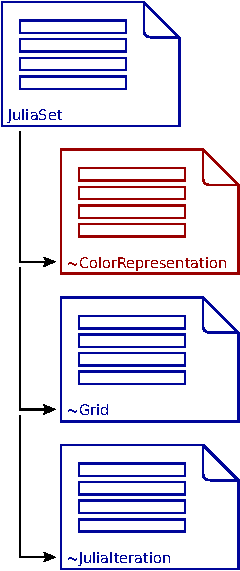
\includegraphics[height=0.8\textheight]{branching_2}
   \end{column}%
   \begin{column}{0.7\textwidth}
    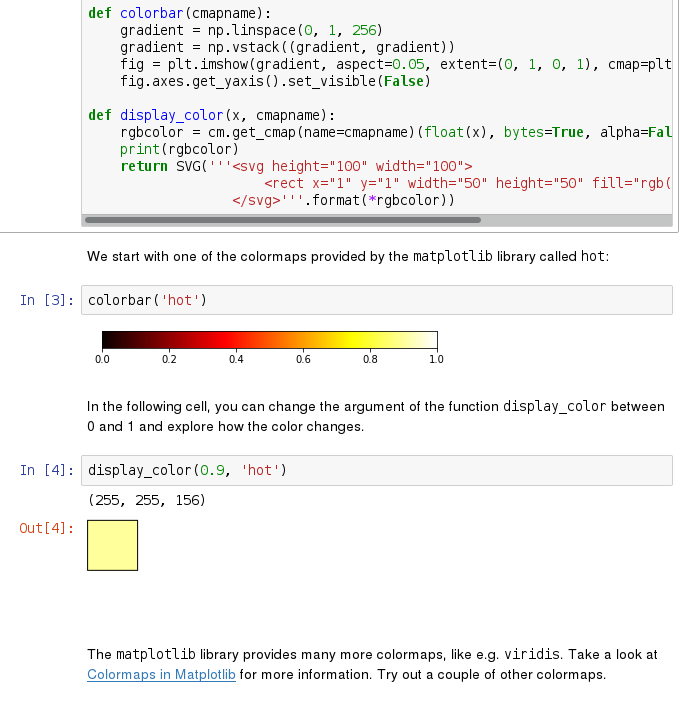
\includegraphics[width=\textwidth]{ColorRepresentation_screenshot}
   \end{column}
  \end{columns}
 }%
 \only<3>{%
  \begin{columns}
   \begin{column}{0.3\textwidth}
    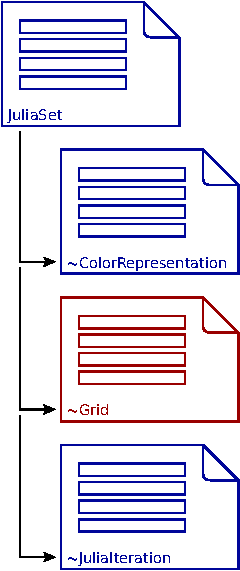
\includegraphics[height=0.8\textheight]{branching_3}
   \end{column}%
   \begin{column}{0.7\textwidth}
    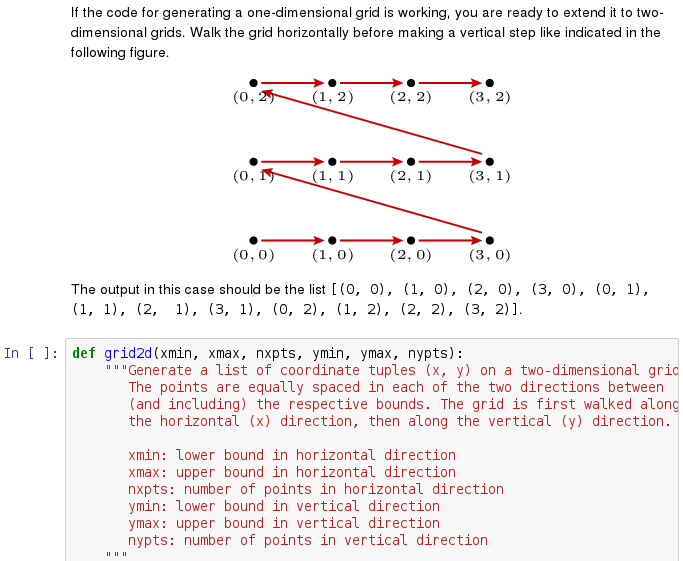
\includegraphics[width=\textwidth]{Grid_screenshot}
   \end{column}
  \end{columns}
 }%
 \only<4>{%
  \begin{columns}
   \begin{column}{0.3\textwidth}
    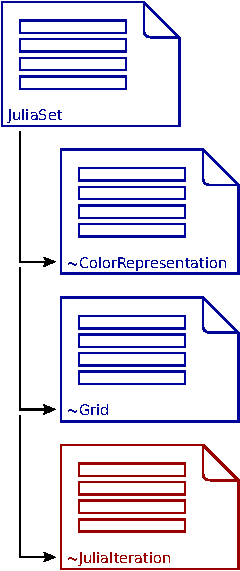
\includegraphics[height=0.8\textheight]{branching_4}
   \end{column}%
   \begin{column}{0.7\textwidth}
    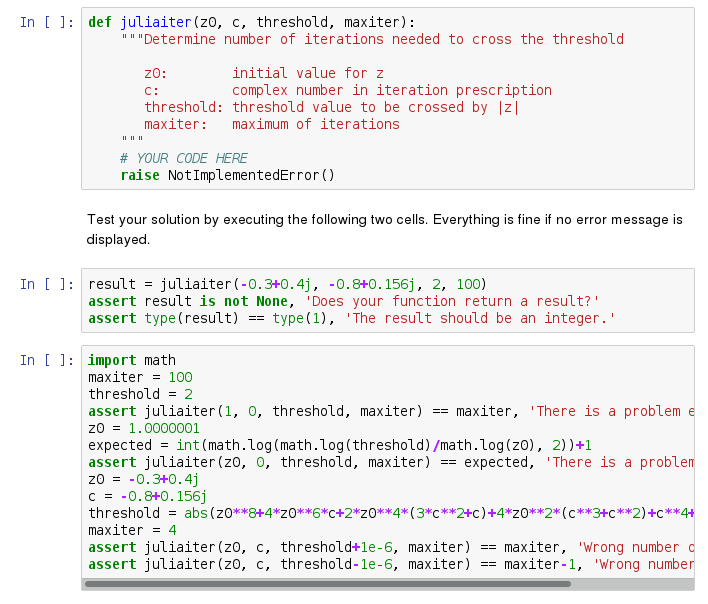
\includegraphics[width=\textwidth]{JuliaIteration_screenshot}
   \end{column}
  \end{columns}
 }%
 \only<5>{%
  \begin{columns}[b]
   \begin{column}{0.3\textwidth}
    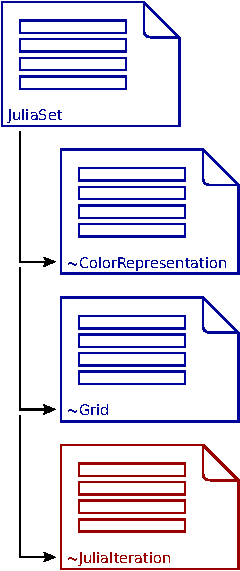
\includegraphics[height=0.8\textheight]{branching_4}
   \end{column}%
   \begin{column}{0.7\textwidth}
    \begin{itemize}
     \item individual path through problem possible
     \item \but notebooks are opened in new tabs, it is easy to lose track
    \end{itemize}

    \vspace{1truecm}
   \end{column}
  \end{columns}
 }
\end{frame}

\end{document}
